\chapter{Web of Data: I Linguaggi}

\section{Introduzione}

\subsection{Perché Studiare il Semantic Web e Linked Data?}

\begin{itemize}
  \item Gli approcci quantitativi non sono sufficienti per domini complessi: 
    \begin{itemize}
      \item Non è possibile apprendere il comportamento giusto per ogni contesto. 
      \item Reattività e ragionamento.
    \end{itemize}
  \item L'ambito della conoscenza è intrinsecamente basato su modelli: 
    \begin{itemize}
      \item Arte, media, tecnologie, etc. 
    \end{itemize}
  \item Interoperabilità dei dati: 
    \begin{itemize}
      \item Conoscenza esperta per stabilire i \fancyglitter{mapping}. 
      \item Utilizzo di standard.
    \end{itemize}
  \item Ruolo nel ragionamento in molte applicazioni: 
    \begin{itemize}
      \item Elaborazione del linguaggio naturale. 
      \item Question answering. 
      \item Chatbots.
    \end{itemize}
\end{itemize}

\subsection{Obiettivi del Corso}

\begin{itemize}
  \item Imparare a rappresentare un dominio di conoscenza con i linguaggi
del Web Semantico (RDF e OWL), che permettono di implementare
ontologie computazionali. 
\item Utilizzare strumenti di ragionamento automatico per realizzare
inferenze sulla conoscenza formalizzata nelle ontologie
computazionali. 
\item Interrogare basi di conoscenza in cui i dati sono rappresentati in un
formato semantico utilizzando il linguaggio SPARQL. 
\item Rendere interoperabili rappresentazioni diverse (ontologie, basi di
dati, fogli di calcolo) utilizzando strumenti di mapping.
\end{itemize}

\section{Dalle Reti Semantiche alle Ontologie}

\subsection{I Limiti della Logica Classica}

A partire dagli anni 60 si è sviluppata una branca
dell’intelligenza artificiale specificamente orientata alla
rappresentazione della conoscenza. Questo rappresenta un tentativo di superare la logica classica allora utilizzata. Il motivo è che la logica classica ha alcuni limiti importanti: 

\begin{itemize}
  \item È caratterizzata da \fancyglitter{inadeguatezza espressiva}.
  \item È \fancyglitter{monotòna}. 
  \item Presenta svantaggi dal punto di vista \fancyglitter{computazionale}.
\end{itemize}

\dfn{Inadeguatezza Espressiva}{
  Alcuni aspetti dell’inadeguatezza della logica classica possono essere
attribuite a differenze con i sistemi cognitivi. 
}

\clm{}{}{
  \begin{itemize}
    \item La logica classica è un \fancyglitter{formalismo piatto}:
      \begin{itemize}
        \item Tutte le affermazioni si collocano sullo stesso piano. 
        \item Esprime conoscenza di carattere generale e immutabile.
      \end{itemize}
    \item Le procedure di dimostrazione sono diverse dal ragionamento umano\footnote{Da premesse false discendono conseguenze vere.}. 
    \item I \fancyglitter{valori di verità} non sono adatti a rappresentare gli aspetti quantitativi
che caratterizzano il mondo reale
  \end{itemize}
}

\dfn{Monotònicità}{
  La logica del primordine è monotòna: le conoscenze inserite
nel sistema logico non possono essere cancellate.
}

\nt{La conoscenza può solo aumentare.}

\clm{}{}{
  \begin{itemize}
    \item Le nuove conoscenze non possono contraddire quelle già
presenti nel sistema. 
\item Impossibilità di rappresentare il cambiamento, quindi gli
aspetti temporali della conoscenza.
  \end{itemize}
}

\dfn{Limitazioni Computazionali}{
  Il calcolo dei predicati è \newfancyglitter{semi-decidibile}: è possibile
dimostrare con certezza cosa discende dalla base di
conoscenza, ma non si ha la certezza di dimostrare ciò che non discende dalla base di conoscenza.
}

\cor{Inefficienza nelle Procedure di Dimostrazione}{
  Per le sue caratteristiche intrinseche (è un formalismo
orientato alla rappresentazione) le procedure di
dimostrazione non sono abbastanza efficienti per le
applicazioni reali.
}

\qs{}{Ma cosa possiamo dire sulle logiche non classiche?}

\paragraph{Le logiche non classiche rilasciano alcune caratteristiche della logica
classica:}
\begin{itemize}
  \item Valori di verità $\Rightarrow$ \fancyglitter{logiche fuzzy}, hanno valori di verità in un intervallo, nascono per superare la rappresentazione binaria dell'informazione.

\begin{figure}[h]
    \centering
    
\includegraphics[scale=0.3]{01/bknb.png}
    \caption{Rappresentazione accurata di una logica fuzzy.}
\end{figure}
\item Conoscenza certa $\Rightarrow$ \fancyglitter{logiche bayesiane}, incorporano il ragionamento probabilistico. 
\item Monotonicità $\Rightarrow$ \fancyglitter{default logics}, belief revision. 
\item Indecidibilità $\Rightarrow$ insiemi decidibili della logica del primordine. 
\item Inefficienza delle dimostrazioni $\Rightarrow$ uso di \fancyglitter{euristiche} nella dimostrazione automatica.
\end{itemize}

\paragraph{Un quadro storico:}

\begin{itemize}
  \item Anni 60s-70s: reti semantiche e frames. 
  \item Anni 70s-80s: logiche non classiche. 
  \item Anni 80s-90s: logiche descrittive. 
  \item Anni 2000s: ontologie computazionali. 
  \item Dal 2010: Linked Data.
\end{itemize}

\subsection{Reti Semantiche}

\dfn{Reti Semantiche}{Le reti semantiche sono:

\begin{itemize}
  \item Basate su una struttura a \newfancyglitter{grafo}. 
  \item I nodi del grafo rappresentano \newfancyglitter{concetti}. 
  \item Gli archi tra i concetti rappresentanole  \newfancyglitter{relazioni tra concetti}.
\end{itemize}
}

\begin{figure}[h]
    \centering
    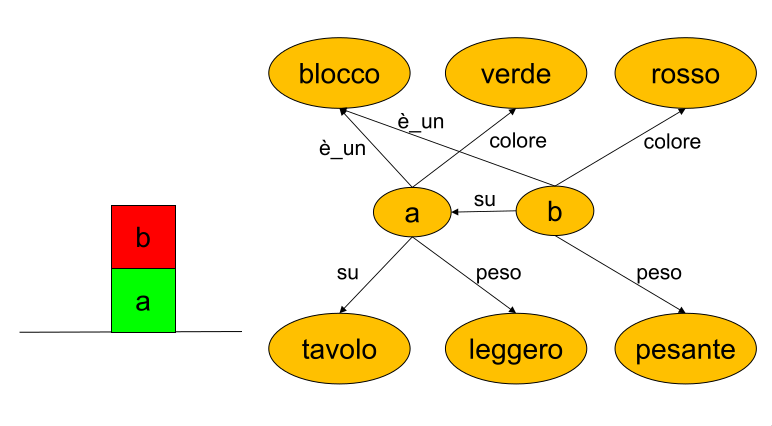
\includegraphics[scale=0.4]{01/grafo.png}
    \caption{Grafo relazionale del "Mondo dei Blocchi", un dominio giocattolo utilizzato nel mondo dell'AI.}
\end{figure}

\nt{Nel "Mondo dei Blocchi" c'è un tavolo su cui è collocato un blocco verde chiamato "a" e sopra un blocco rosso chiamato "b". Una delle possibili rappresentazione è quella dell'immagine in cui sono presenti concetti, qualità ed entità concrete. Gli archi sono varie relazioni.}

\paragraph{Vantaggi di questa rappresentazione:}

\begin{itemize}
  \item Le informazioni relative a un nodo sono \fancyglitter{immediatamente disponibili} dato che ogni blocco è direttamente collegato alle sue proprietà. 
  \item Permette di rappresentare una nozione di \fancyglitter{rilevanza} per cui dato un focus, alcune informazioni si trovano in prossimità. 
\end{itemize}

\paragraph{Corrispondente rappresentazione logica:}

\begin{itemize}
  \item Blocco(a). 
  \item Blocco(b). 
  \item su(b,a). 
  \item su(a,tavolo). 
  \item rosso(b). 
  \item verde(a). 
  \item pesante(b). 
  \item leggero(a).
\end{itemize}

\cor{Ragionamento nelle Reti Semantiche}{
  Nelle reti semantiche il ragionamento consiste nel seguire
un percorso tra nodi.
}

\qs{}{Su quale blocco si trova il blocco b?}

\paragraph{Risposta:} È sufficiente seguire l’arco etichettato come «su» nella rete,
da b verso il nodo a cui punta. Seguendo ulteriormente gli archi si possono inferire relazioni
indirette: il blocco b è "al di sopra" del tavolo.

\subsection{Reti Semantiche e Logica}

L’espressività delle reti semantiche corrisponde a un sottoinsieme della logica del primordine:

\begin{itemize}
  \item Nodi = \fancyglitter{termini}. 
  \item Archi = \fancyglitter{predicati}
\end{itemize}

\begin{figure}[h]
    \centering
    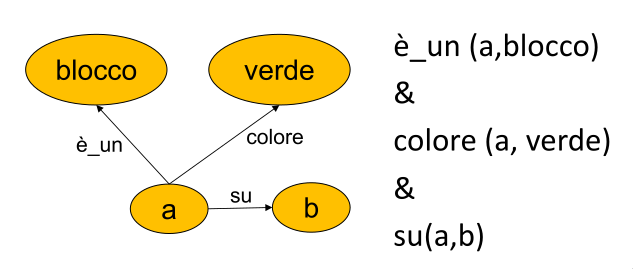
\includegraphics[scale=0.4]{01/grafo2.png}
    \caption{Grafo relazionale in relazionale alla logica del primordine.}
\end{figure}

\nt{Alcune relazioni possono coinvolgere più di due entità.}

\begin{figure}[h]
    \centering
    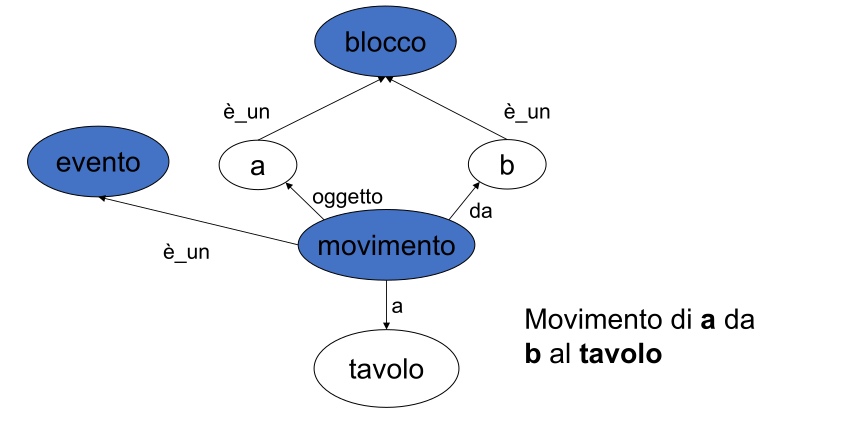
\includegraphics[scale=0.4]{01/grafo3.png}
    \caption{La relazione “movimento” che unisce a, b e tavolo diventa un termine cioè un nodo.}
\end{figure}

\dfn{Reti Semantiche Proposizionali}{
  Le \newfancyglitter{reti semantiche proposizionali} includono nodi che
rappresentano proposizioni. Usando nodi per rappresentare proposizioni è possibile
introdurre una \newfancyglitter{dimensione epistemica}: 
\begin{itemize}
  \item Rappresentare credenze soggettive. 
  \item Lo stesso sistema può rappresentare le credenze di più soggetti
senza che insorgano contraddizioni. 
\end{itemize}
}

\clm{}{}{
  \begin{itemize}
    \item Reti semantiche proposizionali posso avere l’espressività
della logica del primordine una volta introdotti connettivi,
variabili, quantificatori, ecc. 
\item Anche l’inferenza nelle reti proposizionali ha le stesse
caratteristiche che nella logica del primordine. 
\item Soluzione: limitare l’espressività privilegiando tipi di
ragionamento più comuni e computazionalmente trattabili.
  \end{itemize}
}

\dfn{SNePs}{
  Rete semantica proposizionale che incorpora alcuni
elementi della teoria dei frame (Shapiro '79).
}

\nt{Si tratta di una rete semantica con un \fancyglitter{motore di ragionamento}. Permette vari tipi di ragionamento:
\begin{itemize}
  \item Su formule. 
  \item Su slot. 
  \item Su percorsi. 
\end{itemize}
}

\begin{figure}[h]
    \centering
    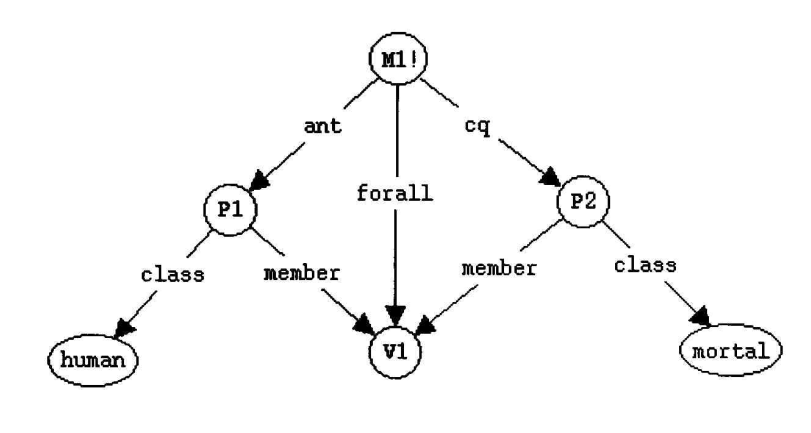
\includegraphics[scale=0.3]{01/socrate.png}
    \caption{Tutti gli uomini sono mortali.}
\end{figure}

\qs{}{Di cosa parla la rete?}

\dfn{Eterogeneità}{
  \begin{itemize}
    \item Archi rappresentano relazioni di tipo diverso tra concetti (relazioni
epistemiche vs fatti). 
\item Nodi rappresentano concetti di tipo diverso (blocco A, blocco)
  \end{itemize}
}

\nt{Alcuni tipi di nodi e di archi sono particolarmente importanti.}

\begin{figure}[h]
    \centering
    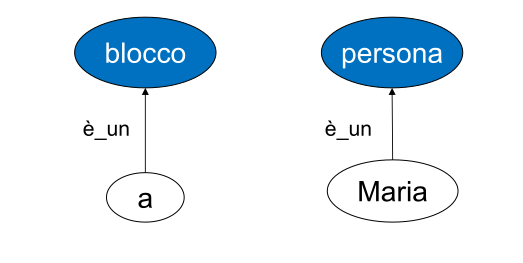
\includegraphics[scale=0.35]{01/node.png}
    \caption{I nodi colorati rappresentano tipi di entità (classi), i nodi bianchi
rappresentano entità singole (individui).}
\end{figure}

\qs{}{"What ISA is and isn't?"}

\begin{itemize}
  \item Gli archi “è un” (IS-A o ISA) hanno un significato diverso
se collegano due classi oppure un individuo a una classe. 
\item Brachman ('83) propone di distinguere i due tipi di
relazioni: “What isa is and isn’t”: 
\begin{itemize}
  \item \fancyglitter{Archi ISA}: appartenenza di una classe a una sottoclasse
(transitiva).
\item \fancyglitter{Archi instance\_of}: appartenenza di un individuo a una classe.
\end{itemize}
\end{itemize}

\begin{figure}[h]
    \centering
    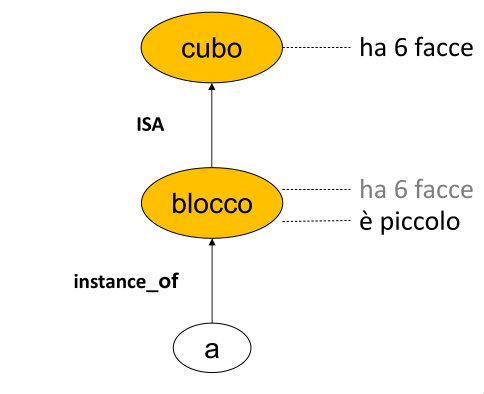
\includegraphics[scale=0.3]{01/ISA.png}
    \caption{ISA e instance\_of.}
\end{figure}

\dfn{Tassonomia}{
  Utilizzando la relazione ISA è possibile esprimere
conoscenza di tipo tassonomico. Si utilizza un ragionamento classificatorio: 
\begin{itemize}
  \item Y è una sottoclasse di Z? $\Rightarrow$ archi ISA. 
  \item x appartiene alla classe Y? $\Rightarrow$ archi instance\_of.
\end{itemize}
}

\begin{figure}[h]
    \centering
    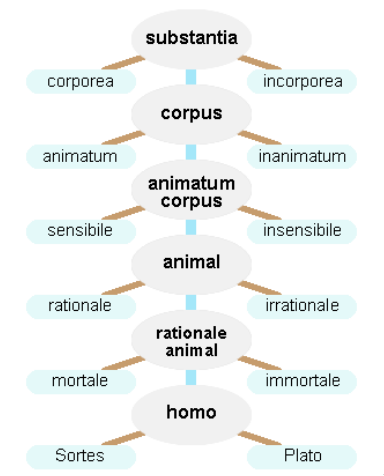
\includegraphics[scale=0.45]{01/porfirio.png}
    \caption{Rappresentazione che deriva dalla filosofia aristotelica, confluita nella scolastica, in cui si raffigurano i principali concetti del pensiero dalla sostanza all'uomo.}
\end{figure}

\nt{Ogni livello \fancyglitter{eredità} le caratteristiche del livello superiore e le caratteristiche non si sovrappongono.}

\paragraph{Vantaggi dell'ereditarietà:}

\begin{itemize}
  \item E’ possibile avere una rappresentazione meno
ridondante facendo una semplice assunzione:
\begin{itemize}
  \item Una classe eredita le proprietà delle classi di cui è sottoclasse. 
  \item Se i cubi hanno sei facce e i dadi sono una sottoclasse dei
cubi, allora anche i dadi hanno sei facce.
\end{itemize}
\item Le sottoclassi hanno proprietà più specifiche delle classi. 
\item Seguendo il percorso degli archi ISA e instance\_of e
diventa possibile ragionare sulle proprietà di un
individuo/classe.
\end{itemize}

\nt{Ma esistono eccezioni, per esempio i pinguini non volano, ma non per questo smettono di essere uccelli. Allo stesso tempo può essere falso per un individuo all'interno di una sottoclasse.}

\dfn{Default Rules}{
  Per gestire le eccezioni è necessario rilasciare la proprietà della
monotonicità (la conoscenza non diminuisce mai). Un esempio è la Default Logic: assunzioni che possono essere
cancellate quando sopravviene nuova conoscenza.
}

\clm{}{}{
  \begin{itemize}
    \item Il trattamento delle eccezioni nelle reti semantiche si basa
sul principio che le conoscenze specificate localmente a un
certo nodo prevalgono su quelle ereditate. 
\item Un corollario è che le conoscenze che comportano meno
passi di inferenza prevalgono su quelle che ne comportano di
più. 
\item Questo principio però non permette di scongiurare tutti gli
inconvenienti.
  \end{itemize}
}

\begin{figure}[h]
    \centering
    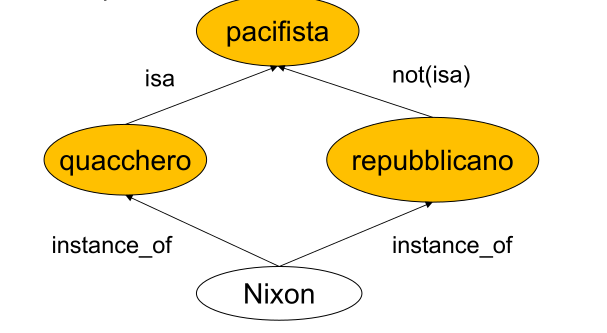
\includegraphics[scale=0.55]{01/nixon.png}
    \caption{Nixon è pacifista o guerrafondaio? In quando quacchero, lo è; in quanto repubblicano,
non lo è (Reiter and Criscuolo, On Interacting Defaults, 1981).}
\end{figure}

\nt{Nemmeno la logica dei default risolve il problema, ciascun default blocca l’altro.}

\dfn{Frame Theory}{
  Evoluzione delle reti semantiche finalizzata a
  rappresentare la conoscenza di tipo stereotipato. Conoscenza di sfondo utile per alcune applicazioni come la \newfancyglitter{visione artificiale} o \newfancyglitter{l’elaborazione del linguaggio}.
}

\dfn{Frame}{
  Un \newfancyglitter{frame} è una struttura dati per la rappresentazione situazioni stereotipate, come trovarsi in una certa tipo di soggiorno o andare al compleanno di un bambino partito. I livelli superiori del telaio sono fissi, e rappresentano cose che sono sempre vere riguardo le situazioni presunte. I livelli inferiori hanno molti terminali: slot che devono essere riempiti da istanze o dati specifici.
}

\cor{Slot}{
  Ogni terminale (slot) può specificare le condizioni che Gli incarichi devono soddisfarsi. (Gli incarichi sono solitamente telai ausiliari più piccoli). Le condizioni possono richiedere un terminale l'incarico di essere una persona, un oggetto ora puntatore a un subframe di un certo tipo. I terminali di un frame sono solitamente riempiti da assegnazioni predefinite. Collezioni di frame collegati sono uniti in frame systems.
}

\paragraph{Struttura di un frame:}

\begin{itemize}
  \item Identificativo. 
  \item Slot: permettono di creare una tassonomia di frame. 
  \item Slot generici: i valori degli slot sono vincolati a un certo tipo, però il contenuto di uno slot può puntare a un altro frame. 
  \item Procedure per il calcolo automatico dei valori. 
  \item Valori predefiniti.
\end{itemize}

\begin{figure}[h]
    \centering
    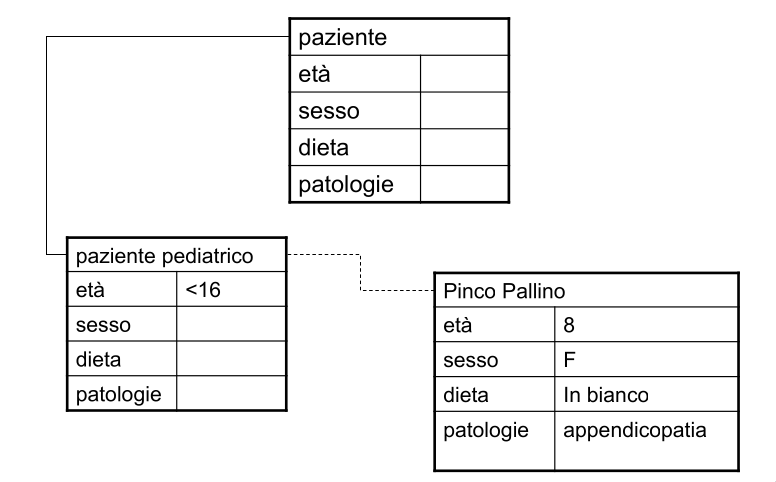
\includegraphics[scale=0.48]{01/tassonomia.png}
    \caption{Esempio di tassonomia.}
\end{figure}

\begin{figure}[h]
    \centering
    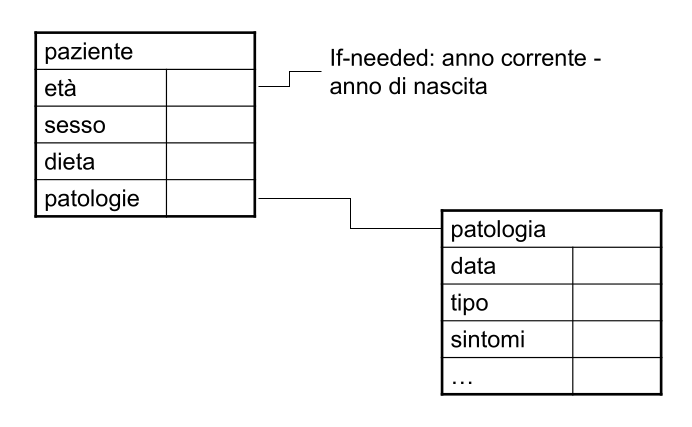
\includegraphics[scale=0.48]{01/non tassonomia.png}
    \caption{Esempio di collegamenti non tassonomici.}
\end{figure}

\dfn{Regole di Produzione}{
  Conoscenza di tipo condizione-azione. Regole IF - THEN (anche dette produzioni): 
  \begin{itemize}
    \item \newfancyglitter{La parte sinistra}: condizioni per l’applicazione delle regola. 
    \item \newfancyglitter{La parte destra}: azioni che sono effettuate se la condizione è
soddisfatta.
  \end{itemize}
}

\clm{}{}{
  \begin{itemize}
    \item Conoscenza dichiarativa: 
      \begin{itemize}
        \item IF allatta(animale,prole) THEN
isa(animale,mammifero). 
\item IF febbre>38,5 and tosse THEN
malattia\_da\_raffreddamento.
      \end{itemize}
    \item Conoscenza procedurale:
      \begin{itemize}
        \item IF intensità(sibilo)>t THEN chiudi(valvola,5mm).
      \end{itemize}
  \end{itemize}
}

\subsection{Sistemi a Regole}

\paragraph{Componenti:}

\begin{itemize}
  \item Base delle regole. 
  \item Memoria di lavoro. 
  \item Interprete delle regole: motore inferenziale. 
\end{itemize}

\paragraph{L'interprete delle regole esegue questo ciclo:}

\begin{enumerate}
  \item Confronto (match) tra fatti (nella memoria di lavoro) e
antecedente delle regole. 
\item Risoluzione di conflitti (più regole applicabili). 
\item Esecuzione (e aggiunta di nuovi fatti alla memoria di lavoro).
\end{enumerate}

\paragraph{Conflitti di applicazione:}

\begin{itemize}
\item \fancyglitter{Refrattarietà}: la stessa regola non viene applicata più volte.
\item \fancyglitter{Recenza}: vengono privilegiate le regole che si applicano ai fatti
più recenti. 
\item \fancyglitter{Specificità}: vengono applicate le regole più specifiche.
\item \fancyglitter{Pesatura}: assegnamento di importanza (peso) a priori alle regole
o ai fatti.
\end{itemize}

\nt{Un passo delicato è il confronto tra la memoria di lavoro e l'antecedente di tutte le regole,}

\dfn{Mycin}{
  Sistema esperto sviluppato a Stanford nei primi anni 70s
(Shortliffe, '75). I fatti sono associati alle probabilità.
}

\begin{figure}[h]
    \centering
    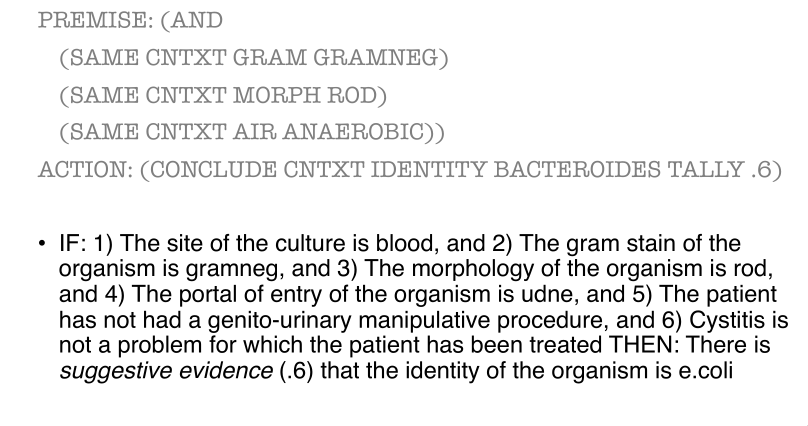
\includegraphics[scale=0.48]{01/mycin.png}
    \caption{Esempio di Mycin.}
\end{figure}






